\documentclass[a4paper,11pt]{article}
\usepackage[utf8]{inputenc}
\usepackage[T1]{fontenc}
\usepackage{lmodern,microtype}
\usepackage[spanish,provide=*]{babel}
\usepackage{amsmath,amssymb,graphicx,float,enumitem,needspace}
\usepackage[margin=2.4cm]{geometry}
\usepackage{xcolor,hyperref,fancyhdr}
\definecolor{deepgreen}{RGB}{23,66,50}
\hypersetup{colorlinks=true,linkcolor=deepgreen,urlcolor=deepgreen,pdftitle={Geometría Axiomática - Lección 1 - Solucionario revisado},pdfauthor={},pdfsubject={Construcciones auxiliares y cálculo de ángulos}}
\pagestyle{fancy}\fancyhf{}\fancyhead[L]{\small Geometría Axiomática}\fancyhead[R]{\small Lección 1 · Solucionario}\fancyfoot[C]{\thepage}
\setlength{\headheight}{14pt}
\setlength{\parindent}{0pt}\setlength{\parskip}{3pt}\setlength{\emergencystretch}{2em}
\usepackage{etoolbox}
\apptocmd{\normalsize}{\setlength{\abovedisplayskip}{5pt}\setlength{\belowdisplayskip}{5pt}\setlength{\abovedisplayshortskip}{4pt}\setlength{\belowdisplayshortskip}{4pt}}{}{}
\normalsize
\newcommand{\tightlist}{\setlength{\itemsep}{0pt}\setlength{\parskip}{0pt}}
\begin{document}
\begin{center}
{\Large\bfseries\color{deepgreen} Geometría Axiomática}\\[5pt]
{\large\bfseries Lección 1 - Solucionario revisado}\\[4pt]
{\small MATG1062 · ESPOL · Material de junio de 2026}
\end{center}
\medskip\hrule\medskip
\textbf{Notación.} \(UV\) denota la longitud del segmento de extremos
\(U,V\) y \(\overrightarrow{UV}\) la semirrecta con origen en \(U\) que
pasa por \(V\), con \(U\ne V\).

\hypertarget{problema-1}{%
\subsection*{Problema 1}\label{problema-1}}

\textbf{Orientación de estudio.} Consulta el libro guía \emph{Classical
Geometry: Euclidean, Transformational, Inversive, and Projective}, de I.
E. Leonard, J. E. Lewis, A. C. F. Liu y G. W. Tokarsky, páginas
\textbf{14 y 15}.

\hypertarget{problema-2}{%
\subsection*{Problema 2}\label{problema-2}}

\hypertarget{datos-de-la-configuraciuxf3n}{%
\subsubsection*{Datos de la
configuración}\label{datos-de-la-configuraciuxf3n}}

Se consideran \(CA=CB=BD\), \(\angle ACB=80^\circ\) y
\(\angle BAD=30^\circ\), con los puntos dispuestos como en la figura. Se
busca

\[x=\angle ABD.\]

\begin{figure}[H]
\centering
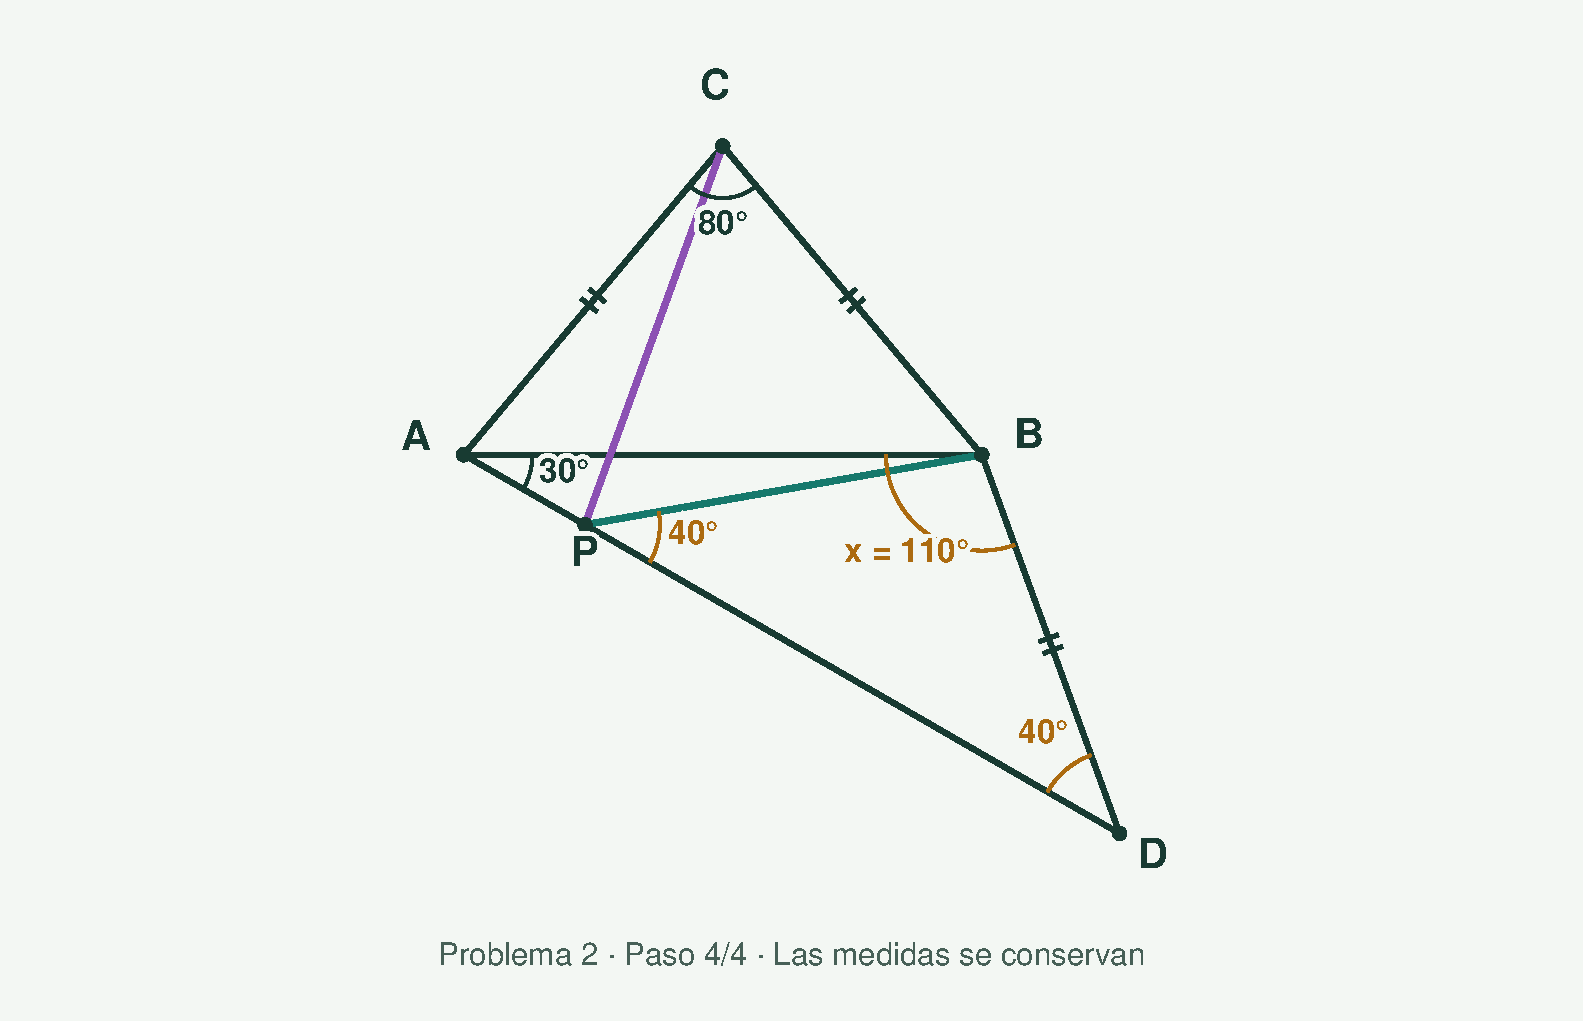
\includegraphics[width=0.9\textwidth]{problem-2-step-4.pdf}
\caption{Construcción auxiliar del problema 2.}
\end{figure}

\hypertarget{construcciuxf3n-del-punto-auxiliar}{%
\subsubsection*{1. Construcción del punto
auxiliar}\label{construcciuxf3n-del-punto-auxiliar}}

Como \(\triangle ABC\) es isósceles y \(\angle ACB=80^\circ\), sus
ángulos de la base son

\[\angle CAB=\angle CBA=\frac{180^\circ-80^\circ}{2}=50^\circ.\]

Dentro de \(\angle ACB\) trazamos una semirrecta que forma \(20^\circ\)
con \(\overrightarrow{CA}\). Sea \(P\) su intersección con
\(\overline{AD}\); en la configuración, los puntos están en el orden
\(A,P,D\). Por construcción,

\[\angle ACP=20^\circ.\]

Además, como \(\overrightarrow{AP}=\overrightarrow{AD}\),

\[\angle CAP=\angle CAB+\angle BAD=50^\circ+30^\circ=80^\circ.\]

En \(\triangle ACP\), la suma de los ángulos interiores da

\[\angle CPA=180^\circ-80^\circ-20^\circ=80^\circ.\]

Los ángulos en \(A\) y \(P\) son iguales. Por el recíproco del teorema
del triángulo isósceles,

\[CA=CP.\]

\hypertarget{un-triuxe1ngulo-equiluxe1tero}{%
\subsubsection*{2. Un triángulo
equilátero}\label{un-triuxe1ngulo-equiluxe1tero}}

Unimos \(B\) con \(P\). Como \(CA=CB\) por hipótesis y \(CA=CP\) por el
paso anterior, se obtiene

\[CP=CB.\]

Por otra parte,

\[\angle BCP=\angle BCA-\angle PCA=80^\circ-20^\circ=60^\circ.\]

Por tanto, \(\triangle BCP\) es isósceles con ángulo del vértice de
\(60^\circ\). Sus otros dos ángulos miden

\[\angle CPB=\angle CBP=\frac{180^\circ-60^\circ}{2}=60^\circ.\]

Así, \(\triangle BCP\) es equilátero y

\[CP=CB=BP.\]

\hypertarget{un-segundo-triuxe1ngulo-isuxf3sceles}{%
\subsubsection*{3. Un segundo triángulo
isósceles}\label{un-segundo-triuxe1ngulo-isuxf3sceles}}

Como \(BD=CB\) por hipótesis y \(BP=CB\), tenemos \(BP=BD\). En
consecuencia, \(\triangle BDP\) es isósceles y

\[\angle BPD=\angle BDP.\]

Dado que \(A,P,D\) están alineados, los ángulos consecutivos en el mismo
semiplano determinado por \(AD\) satisfacen

\[\angle CPA+\angle CPB+\angle BPD=180^\circ.\]

Sustituyendo los valores ya obtenidos,

\[\angle BPD=180^\circ-80^\circ-60^\circ=40^\circ.\]

Por lo tanto, \(\angle BDP=40^\circ\). Como
\(\overrightarrow{DP}=\overrightarrow{DA}\), también

\[\angle BDA=40^\circ.\]

\hypertarget{cuxe1lculo-de-la-incuxf3gnita}{%
\subsubsection*{4. Cálculo de la
incógnita}\label{cuxe1lculo-de-la-incuxf3gnita}}

Finalmente, en \(\triangle ABD\),

\[x+\angle BAD+\angle BDA=180^\circ.\]

De aquí,

\[\boxed{x=180^\circ-30^\circ-40^\circ=110^\circ.}\]

\hypertarget{problema-3}{%
\subsection*{Problema 3}\label{problema-3}}

\hypertarget{datos-de-la-configuraciuxf3n-1}{%
\subsubsection*{Datos de la
configuración}\label{datos-de-la-configuraciuxf3n-1}}

Se consideran \(AB=AD\), \(\angle BAC=40^\circ\),
\(\angle ACD=20^\circ\) y \(\angle ADC=40^\circ\), con la disposición
indicada en la figura. Se busca

\[x=\angle BCA.\]

\begin{figure}[H]
\centering
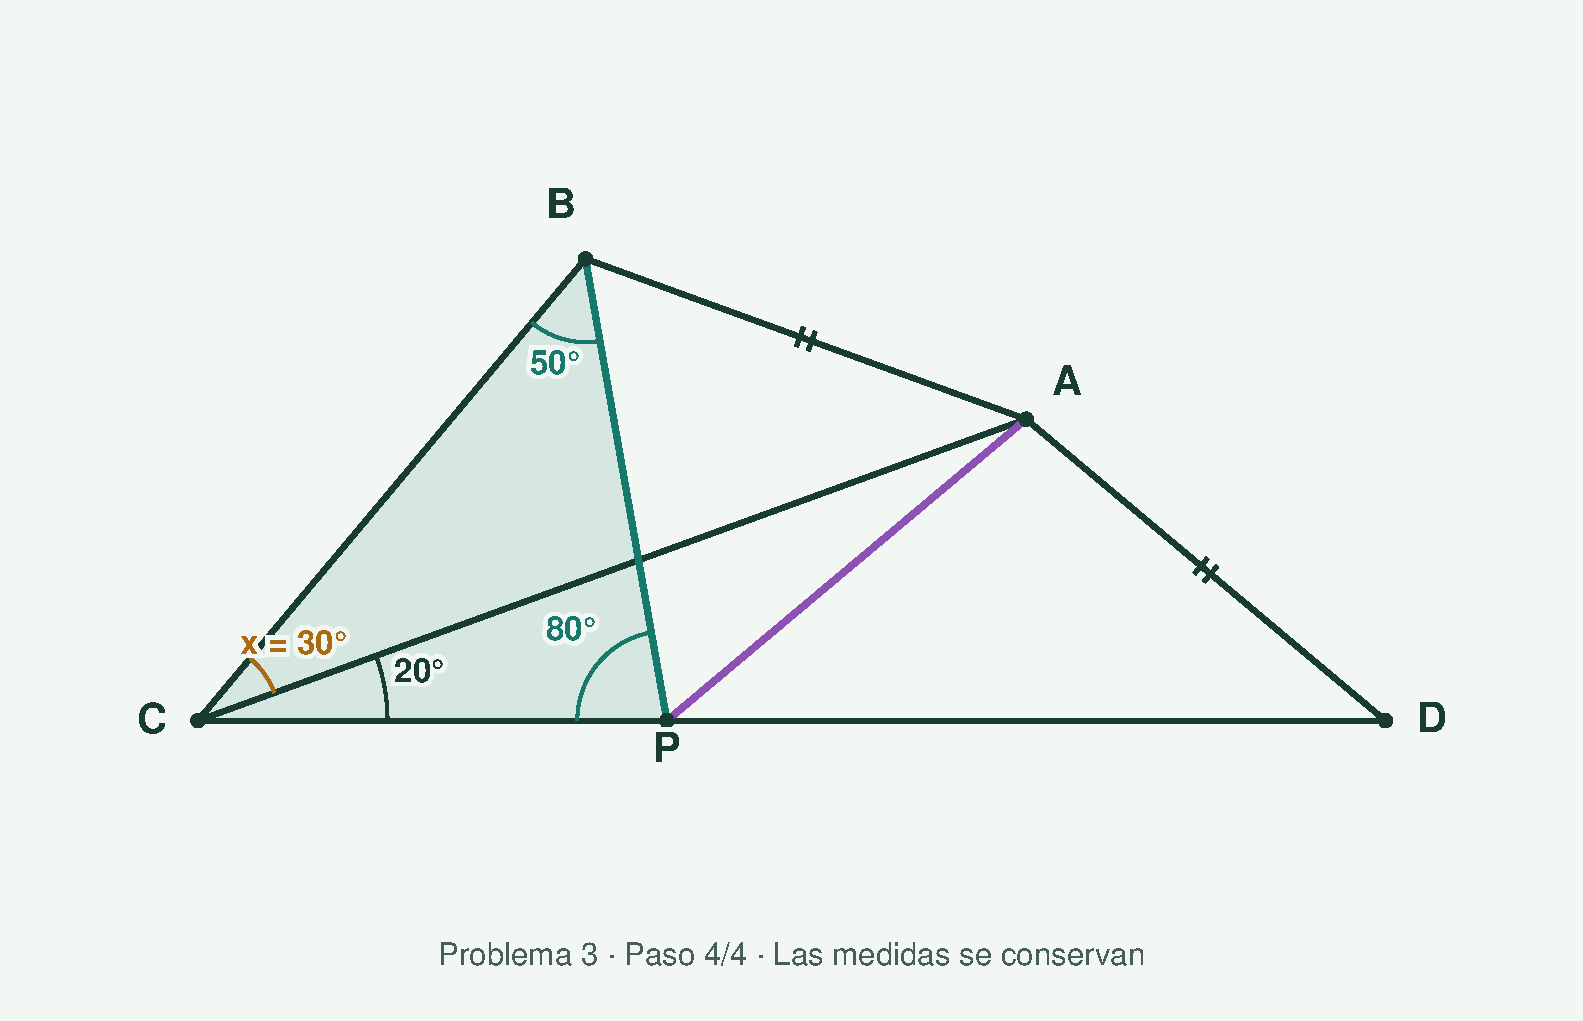
\includegraphics[width=0.9\textwidth]{problem-3-step-4.pdf}
\caption{Construcción auxiliar del problema 3.}
\end{figure}

\hypertarget{construcciuxf3n-del-punto-auxiliar-1}{%
\subsubsection*{1. Construcción del punto
auxiliar}\label{construcciuxf3n-del-punto-auxiliar-1}}

En \(\triangle ACD\),

\[\angle CAD=180^\circ-20^\circ-40^\circ=120^\circ.\]

Dentro de \(\angle CAD\) trazamos una semirrecta que forma \(100^\circ\)
con \(\overrightarrow{AD}\). Sea \(P\) su intersección con
\(\overline{CD}\); los puntos están en el orden \(C,P,D\). Entonces,

\[\angle PAD=100^\circ,\qquad \angle CAP=120^\circ-100^\circ=20^\circ.\]

En \(\triangle ADP\), como \(\overrightarrow{DP}=\overrightarrow{DC}\),

\[\angle ADP=40^\circ.\]

Por la suma de los ángulos interiores,

\[\angle APD=180^\circ-100^\circ-40^\circ=40^\circ.\]

Así, \(\angle APD=\angle ADP\); por el recíproco del teorema del
triángulo isósceles,

\[AP=AD.\]

\hypertarget{un-triuxe1ngulo-equiluxe1tero-1}{%
\subsubsection*{2. Un triángulo
equilátero}\label{un-triuxe1ngulo-equiluxe1tero-1}}

Unimos \(B\) con \(P\). La hipótesis \(AB=AD\) y la igualdad \(AP=AD\)
implican

\[AB=AP.\]

Además,

\[\angle BAP=\angle BAC+\angle CAP=40^\circ+20^\circ=60^\circ.\]

El triángulo \(ABP\) es isósceles con ángulo del vértice de
\(60^\circ\); sus otros dos ángulos también miden \(60^\circ\). Por
consiguiente, es equilátero y

\[AB=AP=BP.\]

\hypertarget{la-igualdad-que-conecta-ambos-triuxe1ngulos}{%
\subsubsection*{3. La igualdad que conecta ambos
triángulos}\label{la-igualdad-que-conecta-ambos-triuxe1ngulos}}

En \(\triangle ACP\) tenemos

\[\angle CAP=20^\circ,\qquad \angle ACP=\angle ACD=20^\circ.\]

Los lados opuestos a estos ángulos son, respectivamente, \(CP\) y
\(AP\). Por tanto,

\[AP=CP.\]

Junto con \(BP=AP\), obtenido en el paso anterior, esto da

\[\boxed{BP=AP=CP.}\]

En particular, \(\triangle BCP\) es isósceles porque \(BP=CP\).

\hypertarget{cuxe1lculo-de-la-incuxf3gnita-1}{%
\subsubsection*{4. Cálculo de la
incógnita}\label{cuxe1lculo-de-la-incuxf3gnita-1}}

Como \(C,P,D\) están alineados, los ángulos consecutivos del semiplano
que contiene a \(A\) y a \(B\) cumplen

\[\angle BPC+\angle APB+\angle APD=180^\circ.\]

Por ello,

\[\angle BPC=180^\circ-60^\circ-40^\circ=80^\circ.\]

Los ángulos de la base del triángulo isósceles \(BCP\) son

\[\angle PBC=\angle PCB=\frac{180^\circ-80^\circ}{2}=50^\circ.\]

Como \(\overrightarrow{CP}=\overrightarrow{CD}\) y \(CA\) queda dentro
de \(\angle PCB\),

\[\angle PCB=\angle BCA+\angle ACD=x+20^\circ.\]

En consecuencia,

\[\boxed{x=50^\circ-20^\circ=30^\circ.}\]

\hypertarget{revision}{%
\subsection*{Para revisar tu razonamiento}\label{revision}}

\begin{itemize}
\tightlist
\item
  Distingue los \textbf{datos} de las igualdades que se demuestran
  durante la solución.
\item
  Si dos ángulos de un triángulo son iguales, identifica con cuidado los
  \textbf{lados opuestos}.
\item
  Antes de sumar ángulos para obtener \(180^\circ\), indica qué puntos
  están alineados y en qué orden se encuentran.
\item
  Girar o reflejar una figura no cambia sus longitudes ni sus ángulos.
  Las imágenes interactivas ayudan a seguir las construcciones, pero no
  sustituyen las demostraciones.
\end{itemize}

\end{document}
